\documentclass[a4paper]{ltxdoc}
\usepackage{lmodern}			% Usa a fonte Latin Modern			
\usepackage[T1]{fontenc}		% seleção de códigos de fonte.
\usepackage[utf8]{inputenc}		% determina a codificação utiizada (conversão automática dos acentos)
\usepackage{hyperref}  			% controla a formação do índice
\usepackage{parskip}			% espaçamento entre os parágrafos
\usepackage{microtype} 			% para melhorias de justificação
\usepackage{morefloats}			% permite mais floats
\usepackage[absolute]{textpos}
\usepackage{tabularx}
\usepackage[table]{xcolor}
\usepackage{graphicx}
\usepackage{mathtools}
\usepackage{multirow}

% Babel e ajustes
\usepackage[english,brazil]{babel}		% idiomas
\addto\captionsbrazil{
  %% ajusta nomes padroes do babel
  \renewcommand{\bibname}{Refer\^encias}
  \renewcommand{\indexname}{\'Indice}
  \renewcommand{\listfigurename}{Lista de ilustra\c{c}\~{o}es}
  \renewcommand{\listtablename}{Lista de tabelas}
  %% ajusta nomes usados com a macro \autoref
  \renewcommand{\pageautorefname}{p\'agina}
  \renewcommand{\sectionautorefname}{se{\c c}\~ao}
  \renewcommand{\subsectionautorefname}{subse{\c c}\~ao}
  \renewcommand{\paragraphautorefname}{par\'agrafo}
  \renewcommand{\subsubsectionautorefname}{subse{\c c}\~ao}
  \renewcommand{\paragraphautorefname}{subse{\c c}\~ao}
}  

\usepackage{color}
\definecolor{thered}{rgb}{0.65,0.04,0.07}
\definecolor{thegreen}{rgb}{0.06,0.44,0.08}
\definecolor{thegrey}{gray}{0.5}
\definecolor{theshade}{rgb}{1,1,0.97}
\definecolor{theframe}{gray}{0.6}
\definecolor{blue}{RGB}{41,5,195}
\newcommand{\orientador}{Prof. Dr. Pedro Paulo Balbi de Oliveira}
\newcommand\tab[1][1cm]{\hspace*{#1}}
\IfFileExists{listings.sty}{
  \usepackage{listings}
  \lstset{%
    language=[LaTeX]TeX,
    columns=flexible,
    basicstyle=\ttfamily\small,
    backgroundcolor=\color{theshade},
    frame=single,
    tabsize=2,
    rulecolor=\color{theframe},
    title=\lstname,
    escapeinside={\%*}{*)},
    breaklines=true,
    commentstyle=\color{thegrey},
    keywords=[0]{\fichacatalografica,\errata,\folhadeaprovacao,\dedicatoria,\agradecimentos,\epigrafe,\resumo,\siglas,\simbolos,\citacao,\alineas,\subalineas,\incisos},
    keywordstyle=[0]\color{thered},
    keywords=[1]{},
    keywordstyle=[1]\color{thegreen},
    breakatwhitespace=true,
    alsoother={0123456789_},
    inputencoding=utf8,
    extendedchars=true,
    literate={á}{{\'a}}1 {ã}{{\~a}}1 {é}{{\'e}}1 {è}{{\`{e}}}1 {ê}{{\^{e}}}1 {ë}{{\¨{e}}}1 {É}{{\'{E}}}1 {Ê}{{\^{E}}}1 {û}{{\^{u}}}1 {ú}{{\'{u}}}1 {â}{{\^{a}}}1 {à}{{\`{a}}}1 {á}{{\'{a}}}1 {ã}{{\~{a}}}1 {Á}{{\'{A}}}1 {Â}{{\^{A}}}1 {Ã}{{\~{A}}}1 {ç}{{\c{c}}}1 {Ç}{{\c{C}}}1 {õ}{{\~{o}}}1 {ó}{{\'{o}}}1 {ô}{{\^{o}}}1 {Õ}{{\~{O}}}1 {Ó}{{\'{O}}}1 {Ô}{{\^{O}}}1 {î}{{\^{i}}}1 {Î}{{\^{I}}}1 {í}{{\'{i}}}1 {Í}{{\~{Í}}}1,
  }
  \let\verbatim\relax
  \lstnewenvironment{verbatim}[1][]{\lstset{##1}}{}
}

\usepackage[alf]{abntex2cite}	% citacoes

\newcommand{\abnTeXSite}{}

\title{\protect\parbox{\textwidth}{\protect\centering \textbf{\titulo}}}

\author{Marcelo Vironda Rozanti\\\abnTeXSite Felipe Stefanelli de Aguiar Silva\\\abnTeXSite} 

\date{\today}

\hypersetup{
  pdftitle={Conservabilidade de estados de autômatos celulares elementares com atualizações assíncronas por prioridade da vizinhança},
  pdfauthor={Marcelo Vironda Rozanti}{Felipe Stefanelli de Aguiar Silva},
  pdfkeywords={Asynchronous priority based updating, Elementary Cellular Automata, New Kind of Science, Discrete dynamical systems, Number-conserving}, 
  pdfproducer={Marcelo Vironda Rozanti},
  pdfcreator={vim+LaTeX+abnTeX2},
  colorlinks=true,
  linkcolor=black,
  citecolor=black,
  urlcolor=blue
}

% \EnableCrossrefs
\CodelineIndex
% \RecordChanges
\hyphenpenalty=1000

\begin{document}

\thispagestyle{empty}
\huge{\centerline{UNIVERSIDADE PRESBITERIANA MACKENZIE}}

\bigskip
\bigskip

\centerline{\large{FACULDADE DE COMPUTAÇÃO E INFORMÁTICA}}

\makeatletter
\vfill
\large{\centering{\@author}}

\vspace*{\fill}

\newcommand{\titulo}{
  \large{\centerline{Dois experimentos com atualização assíncrona por prioridade}}
  \large{\centerline{de vizinhança em autômatos celulares elementares}}
}
\titulo

\vspace*{\fill}
\large{\centerline{SÃO PAULO}}
\large{\centerline{2019}}

\pagebreak

\large{\centering{\@author}}
\vfill
\large{\centerline{\@title}}
\vfill
\vspace*{\fill}

Orientador: \orientador
\\
\\
\\


\large{\centerline{SÃO PAULO}}
\large{\centerline{2019}}

\maketitle

\begin{abstract}
  Autômatos Celulares são sistemas computacionais discretos que se têm provado úteis como modelos genéricos de complexidade e representação de diversas dinâmicas em uma variedade de áreas científicas. Estes sistemas podem ser especificados puramente em termos matemáticos e até implementados em estruturas físicas. Muitos deles podem computar funções e resolver problemas algorítmicos. O presente projeto explora um conjunto fundamental deles, chamados Autômatos Celulares Elementares, com a finalidade de avaliar a conservabilidade no espaço elementar através de um tipo específico de atualização assíncrona, baseada em prioridade da vizinhança.
 % com a esperança de encontrar, no espaço elementar, pares de esquemas de atualização e regras que possam ser usados em aplicações práticas onde haja ambientes dinâmicos que apresentem conservabilidade. 
  % O código correspondende a este trabalho pode ser acessado no repositório \url{https://github.com/mvrozanti/TCC}.
\end{abstract}
Palavras-chave: Autômatos celulares elementares, atualização assíncrona por prioridade da vizinhança, New Kind of Science, Sistemas dinâmicos discretos, Conservabilidade

\vfill

\selectlanguage{english}
\begin{abstract}
  Cellular Automata are discrete computational systems that have proved useful as general models of complexity and representations of dynamics on a variety of scientific fields. These systems can be specified in purely mathematical terms and be implemented in physical structures. Many of them can compute functions and solve algorithmic problems. The present project attempts to explore a fundamental subset of them, called Elementary Cellular Automata with a specific kind of neighbourhood-priority-based asynchronous updating in the search of number-conserving models, which can be used for many practical applications. 
  %The implementation developed is hosted at \url{https://github.com/mvrozanti/TCC}.
\end{abstract}
Keywords: \@pdfkeywords

\break

\selectlanguage{brazil}
\renewcommand{\contentsname}{\centerline{\Large Sumário}}

\tableofcontents

\listoftables

\listoffigures

\break

\section{INTRODUÇÃO}

\tab Autômatos Celulares (ACs) são uma categoria de sistemas discretos. Por sua própria simplicidade, estes sistemas têm ocupado uma posição privilegiada no estudo de complexidade nos mais diversos campos da ciência, de biologia teórica a economia, entre muitos outros. O desenvolvimento de ACs é tipicamente atribuído a John von Neumann através de suas tentativas de criar um modelo abstrato de autoreprodução biológica. Ao fim de 1950, foi notado que ACs poderiam ser vistos como computadores paralelos \cite[p. 876]{wolfram2002new}. Apesar de falta de investigação científica até 1970, um exemplo de AC se tornou muito famoso por seu comportamento complexo e regras simplesmente descritas inventadas por John Conway, \textit{The Game of Life}, que se popularizou após sua aparição na revista \textit{Scientific American}. 

\tab Desde então, múltiplos estudos compreensivos foram realizados por cientistas ao redor do mundo, destacando os trabalhos feitos por Stephen Wolfram na década de 1980, culminando na publicação do livro A New Kind of Science em que Wolfram apresenta uma coleção de resultados a respeito de ACs, com uma série de descobertas revolucionárias. 

% \tab No capítulo \ref{referencial}, é apresentado alguns conceitos básicos referentes à definição dos ACs. 

\subsection{CONTEXTUALIZAÇÃO E RELEVÂNCIA} \label{contex}

\tab A motivação inicial para o estudo de ACs por parte de von Neumann não era matemática mas tinha como diretriz encontrar uma forma viável de tratar do problema de como fazer máquinas se reproduzirem. Hoje é sabido que esses sistemas são aplicáveis para resolver problemas relativos a classificação de densidade, simulação de partículas, compressão de dados, design estrutural, representação de comportamentos dinâmicos como trânsito em cidades ou movimentação de seres vivos entre muitos outros.

\tab Há uma infinidade de ACs passíveis de construção para modelagem ou solução de problemas. Um deles é a modelagem de tráfego de veículos, como é notado por \citeonline[p. 307]{rosenblueth2011model}:  ``Autômatos Celulares Elementares'', discutidos nos próximos capítulos, ``podem modelar tráfego também. Podemos presumir que um veículo se move para frente ou não dependendo apenas na presença ou ausência de outro veículo em sua frente. Supondo que um veículo se move uma célula para a direita se e apenas se uma a célula à direita está vazia, então a regra 184 corresponde ao tráfego se movendo à direita. Movimento aparente é criado do seguinte modo: se o estado de uma célula é 1 e a de seu vizinho à direita é 0, então esta regra atribui 0 ao estado da célula na próxima geração, eliminando o veículo de sua célula atual (que é representada por 110 e 010). Similarmente, se o estado atual da célula é 0 e de seu vizinho à esquerda é 1, então o próximo estado da célula é 1, aparentemente fazendo o veículo no vizinho da esquerda mover-se uma célula para a direita (cobrindo casos 100 e 101). Deve-se lidar com duas outras situações. Primeiro, um veículo não pode se mover se houver outro veículo diretamente em sua frente (i.e., 111 e 011). Segundo, se não há veículo na célula ou seu vizinho à esquerda, então na próxima geração a célula não terá um veículo também (i.e., 001 e 000).''.

\subsection{OBJETO DE PESQUISA} \label{objetopesq}

\tab O objeto de pesquisa deste trabalho são Autômatos Celulares Elementares (ACEs) com atualização assíncrona por prioridade da vizinhança. 

% O primeiro deles se trata de verificar se a regra 184, que é conservativa em modo síncrono, se mantém conservativa em algum esquema de atualização assíncrono, conforme a definição em de conservabilidade detalhada em \ref{num-conserv}. Considerando que é fato conhecido que nenhum AC síncrono é capaz de classificar densidade perfeitamente, o objetivo do segundo experimento foi verificar se algum ACE poderia adquirir essa capacidade em modo assíncrono.

% \tab Dentre o conjunto de esquemas de atualização não-equivalentes, o objetivo é encontrar quais pares $\langle\,R,E\,\rangle$ são conservativos. Dados os esquemas de atualização mencionados na seção \ref{referencial}, encontrar quais esquemas apresentam conservabilidade numérica.

\tab A implementação do simulador tem como parâmetros as seguintes variáveis:

\begin{itemize}
  \item Largura do reticulado:\\
    \tab É o tamanho do reticulado unidimensional, definido como \textit{n}.
  \item Configuração inicial:\\
    \tab Conjunto ordenado de células do AC, cada uma com um estado definido.
  \item Time steps:\\
    \tab Quantidade de reticulados resultantes ou, de iterações da simulação. É a altura das evoluções, para ACEs.
  \item Esquema de prioridades de atualização:\\
    \tab Ordem em que as vizinhanças são atualizadas nas microiterações.
\end{itemize}

Estes conceitos são mais profundamente discutidos no item \ref{referencial}.

\break

\subsection{OBJETIVOS DO ESTUDO} 

% \tab Os objetivos do presente trabalho foram identificar e quantificar pares $\langle\,R,E\,\rangle$ em que há conservabilidade nas evoluções de ACEs com atualização por prioridade da vizinhança. Para alcançar o objetivo geral proposto para a resolução do problema de pesquisa, os seguintes objetivos específicos foram estabelecidos:
O primeiro deles se trata de verificar se a regra 184, que é conservativa em modo síncrono, se mantém conservativa em algum esquema de atualização assíncrono, conforme a definição em de conservabilidade detalhada em \ref{num-conserv}. Considerando que é fato conhecido que nenhum AC síncrono é capaz de classificar densidade perfeitamente, o objetivo do segundo experimento foi verificar se algum ACE poderia adquirir essa capacidade em modo assíncrono.

\begin{itemize}
  \item Definição formal da estratégia de atualização.
  \item Definição de conservabilidade.
  \item Identificação de conservabilidade.
  \item Renderização das evoluções temporais.
  \item Otimização da pesquisa via filtragem de esquemas equivalentes.
\end{itemize}

\subsection{JUSTIFICATIVA}
\tab A motivação para o presente trabalho é explorar em que condições os ACEs são conservativos com o propósito de enumerar evoluções conservativas que podem ser usadas para modelagem de ambientes em que há conservabilidade numérica, questão que será aprofundada no item \ref{referencial}.

\subsection{ORGANIZAÇÃO E DELIMITAÇÃO DO ESTUDO} \label{delimitacao}
\tab A pesquisa se limita a ACEs com o tipo de atualização evidenciado no item \ref{ref_ace}, com largura de reticulados testados até \textit{n}=15 e com \textit{r}=1 e, numa segunda fase, \textit{r}=1.5. Os esquemas de atualização foram filtrados a fim de eliminar esquemas equivalentes, que produzem evoluções idênticas para quaisquer configurações iniciais, de modo que restassem 4683 esquemas no total. Cada esquema contém a prioridade de cada uma das 8 vizinhanças possíveis do espaço elementar, correspondendo às vizinhanças, respectivamente: (111, 110, 101, 100, 011, 010, 001, 000).  Em cada esquema, o número 1 indica que a vizinhança será a primeira a ser atualizada (ou seja, máxima prioridade), o número 2 indica que a vizinhança será a segunda a ser atualizada, e assim por diante. 

% \subsection{ORGANIZAÇÃO DO ESTUDO}

Descrição dos capítulos:

\begin{enumerate}
  \item Introdução
    \subitem Preâmbulo deste trabalho.
  \item Referencial Teórico
    \subitem Sustentação argumentativa sobre o tema proposto.
  \item Metodologia de Pesquisa
    \subitem Sistematização dos instrumentos e processos de estudo empregados no presente trabalho.
  \item Resultados dos Experimentos
    \subitem Análise e apresentação dos resultados das evoluções propostas.
  \item Cronograma
    \subitem Planejamento das tarefas necessárias para a conclusão deste trabalho, bem como suas expectativas de início e conclusão.
\end{enumerate}

\section{REFERENCIAL TEÓRICO} \label{referencial}
\tab Em relação ao referencial teórico estudado neste TCC, foi de suma importância entender os seguintes tópicos:

% \subsection{AUTÔMATOS CELULARES} \label{ref_ac}
\subsection{AUTÔMATOS CELULARES ELEMENTARES} \label{ref_ace}

\tab Um AC pode ser descrito simplesmente por seu \textit{reticulado} e sua \textit{regra de transição}. O reticulado é um conjunto finito \textit{d-dimensional} ordenado de células onde cada célula no índice \textbf{i} tem um estado entre \textit{k} estados. As regras de transição definem o novo estado de uma determinada célula em função de sua vizinhança de tamanho \textit{2r+1}, sendo \textit{r} raio do AC. O comportamento da aplicação das regras de transição nas bordas do espaço pode ser especificado de várias formas, muitas vezes como conexo com a borda oposta, tornando o espaço efetivamente contínuo. 

\tab Uma definição direta das regras de transição consiste na enumeração de todos os estados possíveis da própria célula, das células vizinhas e do próximo estado, contendo a informação necessária para computar o estado futuro das células em função de sua vizinhança e, consequentemente, da evolução como um todo. A regra do AC corresponde a função local, formada por transições de estado. A ação dela sobre cada célula de uma configuração pode ser vista como resultado da ação de uma função global sobre o reticulado, que é distinta da função local.

\begin{figure}[!htbp]
  \centerline{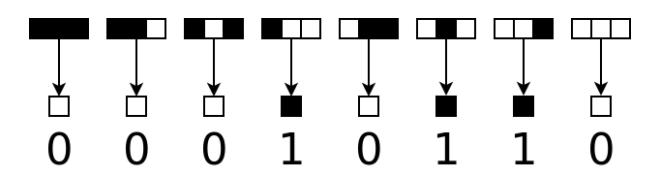
\includegraphics[width=10cm]{imgs/rule_22.png}}
  \caption{Ilustração das regras de transição para a regra 22 no código Wolfram. }
\end{figure}

\tab ACEs formam a família de ACs com \textit{d}=1, \textit{k}=2 e \textit{r}=1, ou seja, são unidimensionais, com células binárias e vizinhanças definidas como 3 células contíguas. O reticulado é dito ter largura \textit{n}, isto é, tem \textit{n} células em cada reticulado da evolução e permanece constante até o fim das evoluções.

\tab Os ACEs são comumente representados por seu respectivo \textit{Wolfram code}, uma nomenclatura que dá a cada regra um identificador no intervalo \(\left[0, 255\right]\). Segundo \citeonline[p. 24]{wolfram2002new}, ``A linha superior em cada caixa dá uma das possíveis combinações de cores para uma célula e sua vizinhança imediata. A linha inferior então especifica qual será a cor da célula central no próximo passo em cada um desses casos.''

\begin{figure}[!htbp]
  \centerline{
\includegraphics[width=8cm]{imgs/256ecas.png}}
  \caption{Ilustração das 256 regras elementares. }
\end{figure}

\break
\subsubsection{ATUALIZAÇÃO ASSÍNCRONA \\POR PRIORIDADE DA VIZINHANÇA} \label{tiposatt}
\tab Parte imprescindível da definição de um AC é a ordem de atualização das células no reticulado. Apesar de os ACs serem fundamentalmente concebidos com o comportamento de atualização síncrona, é possível se utilizar das mais diversas e criativas estratégias de atualização.

\tab No presente trabalho foi empregado um tipo inédito de estratégia de atualização: em função da prioridade da vizinhança, que consiste em cada uma das 8 regras de transição estar associada a uma prioridade no intervalo \(\left[1, 8\right]\), (e.g.: 12344321). Esse tipo de atualização requer uma distinção das iterações globais e locais (microiterações):  as prioridades de vizinhanças são iteradas sequencialmente de menor a maior e para cada prioridade, o reticulado é varrido e atualizam-se apenas as células que tenham vizinhança com a prioridade atual, mantendo-se o estado das vizinhanças que não estejam na prioridade atual da iteração. Ao fim da varredura do reticulado, o processo se repete para a próxima prioridade, agora iterando sobre o reticulado gerado no processo descrito anteriormente. O reticulado resultante após iterar sobre todas as prioridades é chamado de iteração global (ou macroiteração) e é incluído nas renderizações, o que não acontece com as microiterações.

\tab Esse modo de atualização inclui também a atualização síncrona, que pode ser simulada quando as prioridades do esquema têm mesmo valor (11111111, 22222222, ..., etc). Diferentes esquemas de prioridade aplicados a uma mesma regra podem gerar evoluções equivalentes para quaisquer configurações iniciais. Estes esquemas são chamados esquemas equivalentes. As evoluções podem ser identificadas como um par $\langle\,R,E\,\rangle$, onde \textit{R} é a regra e \textit{E} é um esquema de prioridade. 

\tab No presente trabalho, são filtrados os esquemas simetricamente equivalentes, isto é, os esquemas semi-totalísticos: ``Regras totalísticas dependem apenas do número total de células pretas em uma vizinhança; regras semi-totalísticas [...] também dependem da cor da célula central'' de acordo com \citeonline{wolfram2002new}. Para ACEs, é possível gerar 1.194.165 combinações de pares $\langle\,R,E\,\rangle$. 

% \break 
\subsection{CONSERVABILIDADE NUMÉRICA} \label{num-conserv}
\tab Segundo \citeonline{boccara2002number}, ``Uma regra de AC \textit{f} de \textit{q} estados, unidimensional, de largura \textit{n} é conservativa se, para todas as configurações cíclicas de tamanho \textit{L} \(\geq\) \textit{n} satisfaz'':

\[f(x_1,x_2,...,x_{n-1},x_n) + f(x_2,x_3,...,x_n,x_{n+1}) + ... \]
\tab \[ + \;   f(x_L,x_1,...,x_{n-2},x_{n-1} = x_1 + x_2 + ... + x_L\] 

% \break

\tab No contexto de ACEs, uma evolução é dita conservativa caso, para qualquer configuração inicial, a quantidade de um determinado estado é sempre a mesma para todas as iterações. Como é mencionado no item \ref{contex}, ACs conservativos podem ser usados para modelar ambientes em que há conservabilidade, como trânsito automobilístico, simulação de partículas, entre outros. A regra 184 é uma regra que, com execução síncrona e (como este trabalho apresenta) assíncrona, gera evoluções conservativas pela definição anterior de conservabilidade.

\section{METODOLOGIA DA PESQUISA}
\tab No que tange à Metodologia empregada neste TCC, o trabalho teve início com uma revisão da literatura específica sobre o tema da pesquisa. Esta pesquisa abrange conceitos fundamentais de teoria da computação e o ``estado da arte'' em termos de análise de conservabilidade.

\tab Este alicerce teórico foi obtido através de autores como: Wolfram; Boccara;
entre outros, além de pesquisas em periódicos científicos, sites, publicações em empresas, teses e dissertações em universidades e publicações de associações técnicas.  A leitura, análise e comparação da fundamentação teórica tiveram início com ACEs síncronos, modificados em seguida para viabilizar o tipo de atualização mencionado no item \ref{tiposatt}.

\subsection{ETAPAS DA PESQUISA}
\tab Para definir as etapas da pesquisa, foi necessário examinar as delimitações de estudo (item \ref{delimitacao}), desenvolvendo uma implementação que atendesse à execução dos ACE com esquemas totalmente distintos, como descrito no Cronograma apresentado no item \ref{cron}. No decorrer da fundamentação teórica foram realizados experimentos para verificação de conservabilidade inicialmente em modo de atualização síncrona e então assíncrona, com o objetivo de verificar conservabilidade. 

\tab Os 4683 esquemas de atualização mencionados no item \ref{ref_ace} foram testados primeiramente contra a regra 184, que é conservativa em modo síncrono. A extensão de evoluções celulares se limitou a n=15, como é explicitado no item \ref{delimitacao}.

% \break

Assim, pode-se dizer que as etapas desenvolvidas neste estudo foram:

\begin{enumerate}
  \item Revisão bibliográfica;
  \item Fundamentação teórica;
  \item Desenvolvimento e implementação em Python;
  \item Simulação;
  \item Análise das simulações;
  \item Conclusão e documentação final da pesquisa.
\end{enumerate}

\subsection{CLASSIFICAÇÃO DA PESQUISA}
\tab O tempo total previsto para a conclusão desta pesquisa é de 1 ano, como mostrado no capítulo \ref{cron}.

\tab Esta é uma pesquisa exploratória, dada a natureza desconhecida das propriedades de ACEs com o tipo de atualização mencionado em \ref{ref_ace}. Baseada em medidas objetivas e dados verificáveis, esta pesquisa foi voltada para encontrar caminhos, formas, maneiras e procedimentos para atingir um determinado fim, buscando definir um processo ou uma ferramenta que leve à solução do problema proposto.  Quanto aos meios, foram utilizados os recursos mencionados na Bibliografia.

\break

\section{RESULTADOS DOS EXPERIMENTOS}

A simulação da regra 184 para todos os esquemas de prioridade não-equivalentes até largura \textit{n}=15 mostra em quais esquemas a regra permanece conservativa:

\begin{figure}[h]
  \begin{minipage}[htb]{.4\linewidth}
    \centering
    \fbox{
\includegraphics[width=0.1\linewidth]{imgs/184-5x33-11111111.png}}
    \caption{As evoluções geradas por esses pares $\langle\,R,E\,\rangle$ são idênticas}
    \label{fig:evolucoes}
    % \rule{6cm}{6cm} %to simulate an actual figure
  \end{minipage}%
  \begin{minipage}[htb]{.6\linewidth}
    \centering
    \begin{tabular}{ | c | c | } \hline
      Regra & Esquema  \\\hline 
      \multirow{13}{*}{184} 
	    & \underline{3}222\underline{2}2\underline{21} \\
	    & \underline{3}111\underline{1}1\underline{12} \\      
	    & \underline{2}333\underline{3}3\underline{31} \\      
	    & \underline{2}111\underline{1}1\underline{13} \\      
	    & \underline{1}333\underline{3}3\underline{32} \\      
	    & \underline{1}222\underline{2}2\underline{23} \\      
	    & \underline{2}222\underline{2}2\underline{21} \\      
	    & \underline{2}111\underline{1}1\underline{12} \\      
	    & \underline{2}111\underline{1}1\underline{11} \\      
	    & \underline{1}222\underline{2}2\underline{22} \\      
	    & \underline{1}222\underline{2}2\underline{21} \\      
	    & \underline{1}111\underline{1}1\underline{12} \\      
	    & \underline{1}111\underline{1}1\underline{11} \\       
      \hline
    \end{tabular}
\end{minipage}
\label{fig:test}
\end{figure}

\tab As prioridades com underscore significam que qualquer prioridade pode ser colocada em seu lugar. Isto se deve a, nesses índices, as transições de estado serem não-ativas e, portanto, serem irrelevantes em que ordem são atualizadas.
No entanto, é possível ver que as prioridades das transições de estado ativas são iguais entre si, que são todas representações equivalentes da execução síncrona.

\tab A seguir será apresentadada a análise dos ACEs com o tipo de atualização proposto para \textit{r}=1.5.

\break

\section{CRONOGRAMA} \label{cron}

\tab As atividades desta pesquisa se desenvolveram de acordo com o cronograma apresentado a seguir, no prazo de 12 meses:

\newcommand{\ccy}{\cellcolor{yellow}}
\begin{table}[h]
  \caption{Cronograma de atividades}
  \centerline{
    \begin{tabular}{|l|l|l|l|l|l|l|l|l|l|l|l|l|} \hline
      \multirow{2}{*}{ATIVIDADE}                & \multicolumn{12}{|c|}{MÊS}     						    \\
				                & 1    & 2    & 3    & 4    & 5    & 6    & 7    & 8    & 9    & 10   & 11   & 12   \\\hline
      Revisão bibliográfica                             
						& \ccy & \ccy &      &      &      &      &      & \ccy &      &      &      &      \\\hline
      Fundamentação teórica                             
						&      & \ccy & \ccy &      &      &      &      &      &      &      &      &      \\\hline
      Desenvolvimento e implementação em Python         
						&      & \ccy & \ccy &      &      &      &      &      &      &      &      &      \\\hline
      Conclusão e documentação final da pesquisa        
						&      &      &      & \ccy & \ccy &      &      &      &      &      &      &      \\\hline
      Experimento 1                        
						&      &      &      & \ccy & \ccy &      &      &      &      &      &      &      \\\hline
      Experimento 2                      
						&      &      &      &      &      & \ccy & \ccy &      &      &      &      &      \\\hline
      Análise e validação dos experimentos                            
						&      &      &      &      &      & \ccy & \ccy &      &      &      &      &      \\\hline
      Conclusão e documentação final da pesquisa        
						&      &      &      &      &      &      &      & \ccy & \ccy & \ccy & \ccy & \ccy \\\hline
    \end{tabular}
  }
\end{table}

% \break

\addcontentsline{toc}{section}{Referências}
\bibliography{cellz} \label{bib}

\end{document}
